\section{Architecture}
\subsection{von Neumann}
\begin{figure}[!htb]
	\center{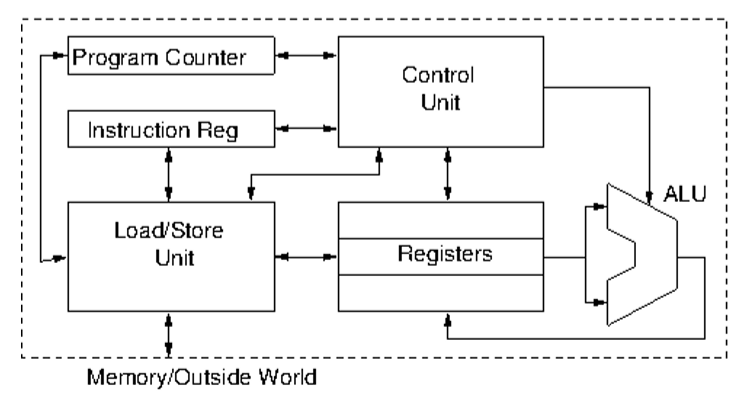
\includegraphics[width=9cm]
		{csa/vonover}}
	\caption{\label{fig:vonover} von Neumann Overview}
\end{figure}
von Neumann architecture is the more common CPU architecture used in modern times. There are a few components, as seen in the figure, and they each serve their unique purpose.
\begin{enumerate}
	\item Main Memory: Logically seperate from the CPU; it holds all the instructions and data that make up a program. This data is stored in distinct locations, referred to as "memory addresses."
	\item Load/Store Unit: The interface between the CPU and the outside world; transfers data via the bus.
	\item Registers: Local, fast storage that holds data currently in use. Each register holds one "word" of data. Does not hold instructions.
	\item Instruction Register: Holds instruction. This is used by the control unit to configure the ALU. In usual design, only one instruction is active at any given time.
	\item ALU: Arithmetic Logic Unit; where computations take place. Reads data from registers and writes results back into registers.
	\item Program Counter: Special register that contains the memory address of the next instruction to execute.
	\item Extra:
	\begin{enumerate}
		\item Cache: Intermediate memory between CPU and Main Memory used for fast access of external memory
		\item IO Controller: Handles peripheral devices via an extension of memory addressing protocol or interrupt-based protocol. Connects via bus.
	\end{enumerate}
\end{enumerate}
memory, load/store unit, registers, instruction register, alu, program counter, 

\subsection{Execution}
\paragraph{Fetch-Decode-Execute}
\begin{enumerate}
	\item Inspect the program counter to find the address of the next instruction
	\item Load the next instruction from memory into the instruction register
	\item Update the program counter to point at the next instruction
	\item Determine the type of instruction fetched
	\item If the instruction requires data from memory, determine its address
	\item Fetch any required data from memory into one of the CPU registers
	\item Execute the instruction
	\item Return to step 1 for next instruction
\end{enumerate}

\subsection{CPI and Execution Time}
\paragraph{CPI} CPI is the average clock cycles per instruction. CPU processer speeds are calculated as cycles per second. To find CPI, you simple take the total number of cycles $IC*CC$ and divide by the total number of instructions $IC$. Giving us the formula: \[CPI = \frac{\sum_{i}*IC_i*CC_i}{IC}\].
\paragraph{Clock Time} 
\paragraph{MIPS} Millions of Instruction Per Second is what MIPS stands for. To get this value, find the clock frequency and divide it by 1 million multiplied with the CPI. \[MIPS = \frac{CPU (Hz)}{CPI*1,000,000}\]
\paragraph{Execution Time} To find execution time, the total time it takes to execute the instruction, we simply multiply CPI, IC and the clock time (or divide by clock frequency). \[ET = \frac{CPI *IC}{CPU (Hz)}\]
\section{MIPS Microarchitecture}
This section deals with the MIPS microarchitecture and how to construct it.
\begin{itemize}
	\item Microarchitecture: Detailed structure and organisation of the machine.
	\item Datapath: Collection of functional units which implement the instruction set.
	\item Control Logic: Configures the datapath in the correct way so that it implements the desired instruction.
\end{itemize}
\subsection{Building Datapaths}
\paragraph{Instruction Fetch}
The first step of the instruction cycle is to get the address of the next instruction and then fetch the instruction itself. To do this, we must send the contents of the program counter to memory, as an address, and bring the contents of that address into the CPU as the next instruction. We will need the Program Counter, Main Memoru (usually physically off-chip) and an Instruction Register. We will also need an "adder" of sorts to increment the Program Counter. 
\begin{figure}[!htb]
	\center{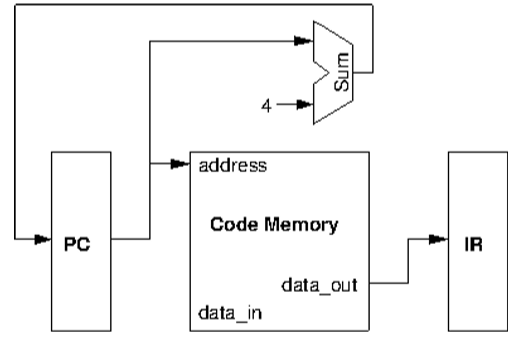
\includegraphics[width=7cm]
		{csa/mipsinstruct}}
	\caption{\label{fig:mips1} Instruction Fetch datapath sketch}
\end{figure}
\paragraph{R-Type Instruction}
R-Type instructions are instructions where all data values used are in the register. Each 32-bit R-Type instruction is partitioned as follows:
\begin{itemize}
	\item 6-bits: Opcode (machinecode representation of the instruction)
	\item 5-bits: Source 1
	\item 5-bits: Source 2
	\item 5-bits: Destination
	\item 5-bits: Shift
	\item 6-bits: Funct (For instructions that share an opcode, the funct parameter contains the necessary control codes to differentiate the different instructions.)
\end{itemize}
As such, 15 of these bits are dedicated to selecting registers that are involved in ALU computations.
\begin{figure}[!htb]
	\center{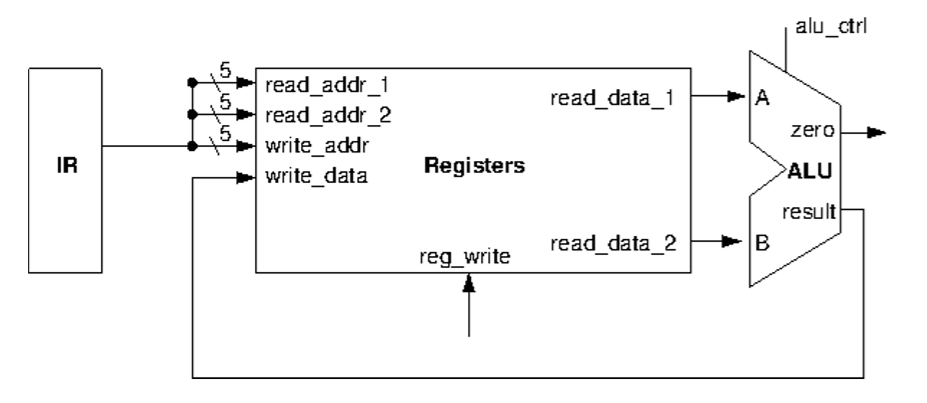
\includegraphics[width=10cm]
		{csa/rtype}}
	\caption{\label{fig:rtype} R-Type instruction datapath}
\end{figure}

\paragraph{Load/Store Instruction}
Load/Store Operations are more complex than ALU instructions; they need to have R/W access to registers, memory and be able to use the ALU to calculate addresses.
\begin{itemize}
	\item 6-bits: Opcode
	\item 5-bits: Base Address (Register containing such address)
	\item 5-bits: Source/Destination (Register containing such address)
	\item 16-bits: Address Offset
\end{itemize}
\begin{verbatim}
lw $t0, 8($sp)
\end{verbatim}
In this example, lw is the opcode, \$t0 is the destination, \$sp is the base address, and 8 is the offset.
One thing to note, is that the address offset is 16 bits, but the ALU processes values at 32-bits. Due to how we represent negative values, and the fact we want to be able to offset in the negative, we will need a Sign Extension Unit to increase our offset to 32-bits before moving it to the ALU.
\begin{figure}[!htb]
	\center{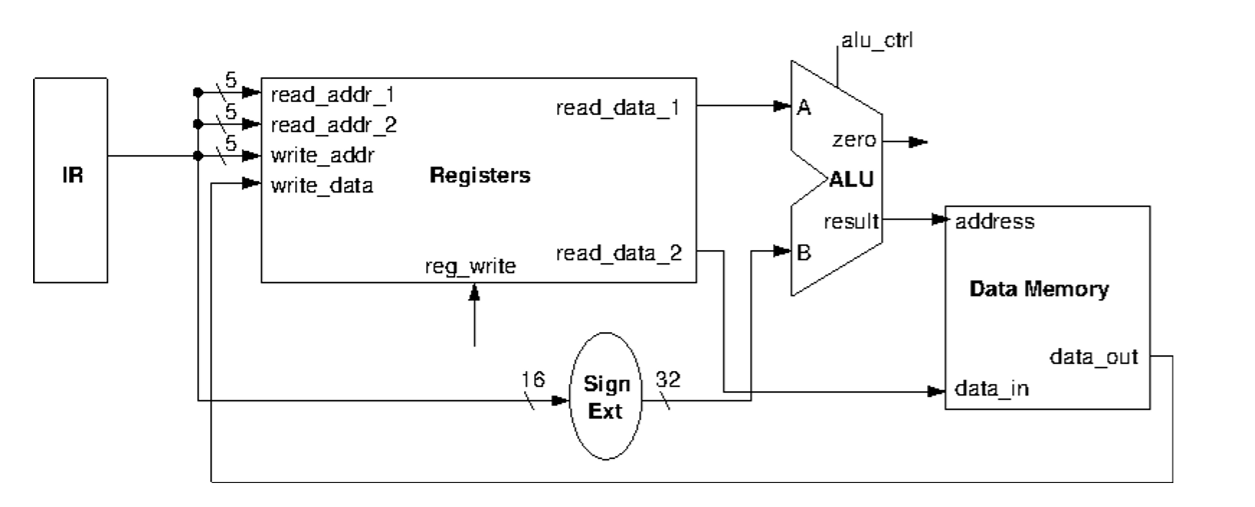
\includegraphics[width=12cm]
		{csa/loadstore}}
	\caption{\label{fig:loadstore} Load/Store Operations Datapath}
\end{figure}
\paragraph{Branches and Jumps}
Branches and jumps essentially achieve the same result; they must both be able to change the contents of the program counter. However, branches require a comparison to be done beforehand, whereas a jump does not. Jumps are a small addition to the structure of a branch datapath, so lets look at branches first.
\begin{itemize}
	\item 6-bits: Opcode
	\item 5-bits: Base Address (Register containing such address)
	\item 5-bits: Source/Destination (Register containing such address)
	\item 16-bits: Address Offset
\end{itemize}
This is the same instruction structure as Load/Store. However, instead of accessing the memory to, well, load/store, it instead needs to add/increment the PC. This is shown in the diagram.
\begin{figure}[!htb]
	\center{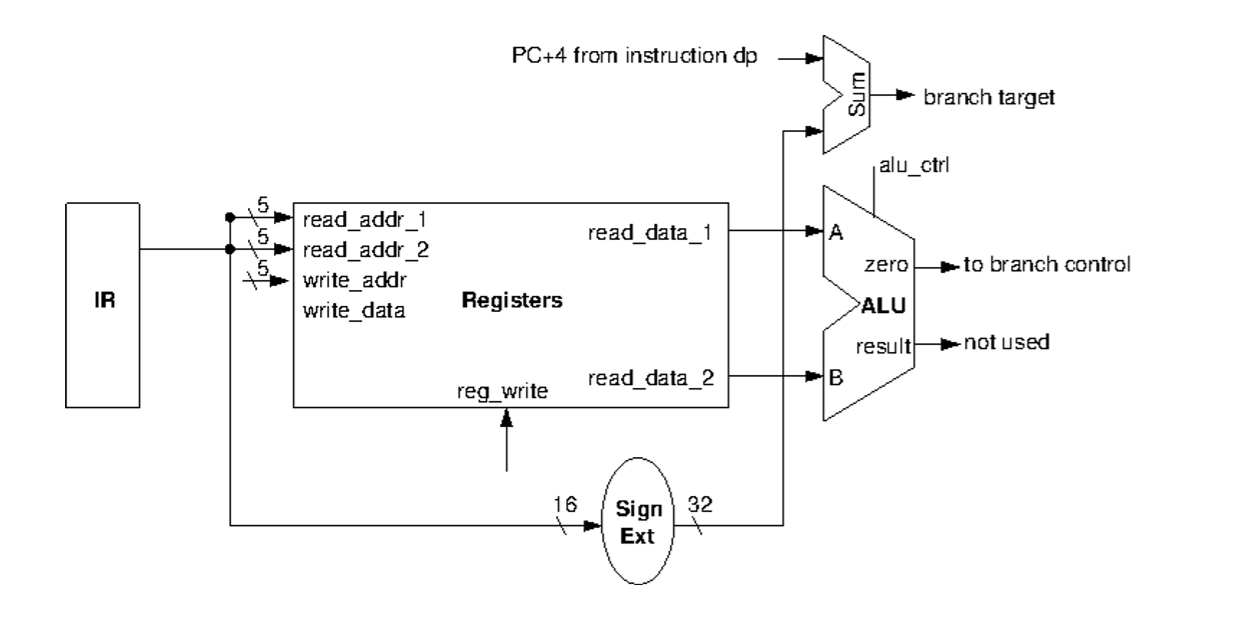
\includegraphics[width=14cm]
		{csa/branch}}
	\caption{\label{fig:branch} Branch Instruction Datapath}
\end{figure}
\paragraph{Multiplexing}
As you can see, the different instruction can use the same components. This is a problem if we want to combine them into one big boy datapath. To do this, we use a technique known as multiplexing. Multiplexers allow us to transmit multiple signals along the same channel, selecting which one to pass. A multiplexer has three sets of wires, an input, an output, and a control. For every $N$ control wires, we can choose between $2^N$ inputs, so a 2-1 multiplexer has 1 control, a 4-1 has 2 control, an 8-1 has 3 control, etc. Let's look at this one bit multiplexer example;
\begin{verbatim}
if (C==0)
    Q = x + y;
else
    Q = x + z;
\end{verbatim}

 \begin{figure}[!htb]
 	\center{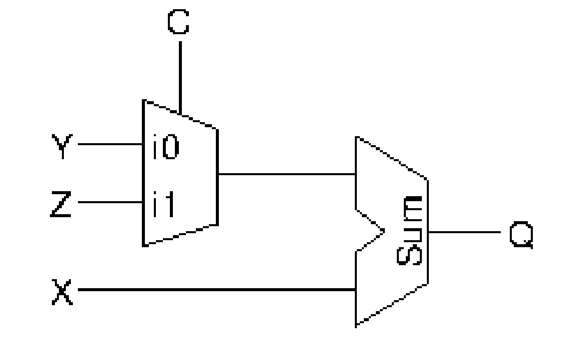
\includegraphics[width=6cm]
 		{csa/multiplex}}
 	\caption{\label{fig:multiplex} Multiplexer Example}
 \end{figure}
\subsection{Combining Datapaths}
\paragraph{ALU and Load/Store}
In an ALU instruction, both inputs to the ALU are from the registers, and the registers provides data to just the ALU. In a Load/Store instruction, the second ALU input is from the sign extender, and the data written to a register is from the Data Memory. We will need two multiplexers and two control lines, referred to as \textbf{alu\_src} for the ALU input and \textbf{mem\_to\_reg} for the register writing.
\begin{figure}[!htb]
	\center{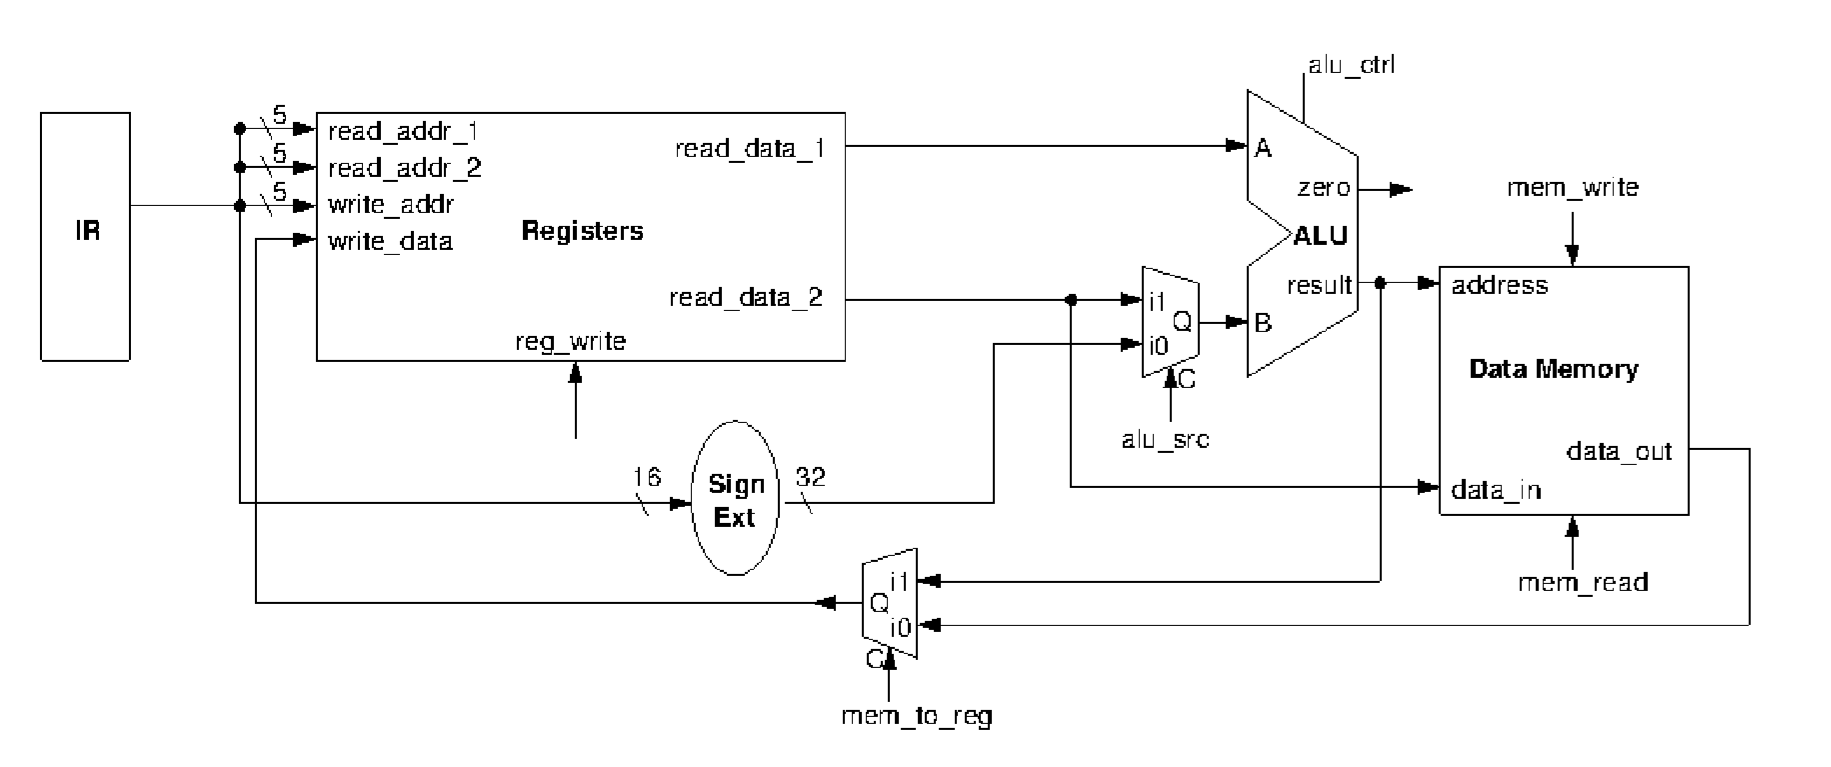
\includegraphics[width=17cm]
		{csa/aluls}}
	\caption{\label{fig:aluls} ALU and Load/Store Integration}
\end{figure}
\paragraph{Instruction Fetch  and Branches}
Instruction fetch doesn't use any of the same resources as ALU or Load/Store instructions, so it's easy to integrate. We will look into integrating branches with them. Either the PC incremented with 4 is set as the new PC, or the added branch offset is added. 2 to 1 can only mean one thing, multiplexing. A multiplexer is added after the second adder component from the branch datapath, using a \textbf{pc\_src} control wire. The rest of the components in the branch datapath are not unique to it, and does not require any other changes or multiplexing.
 \begin{figure}[!htb]
	\center{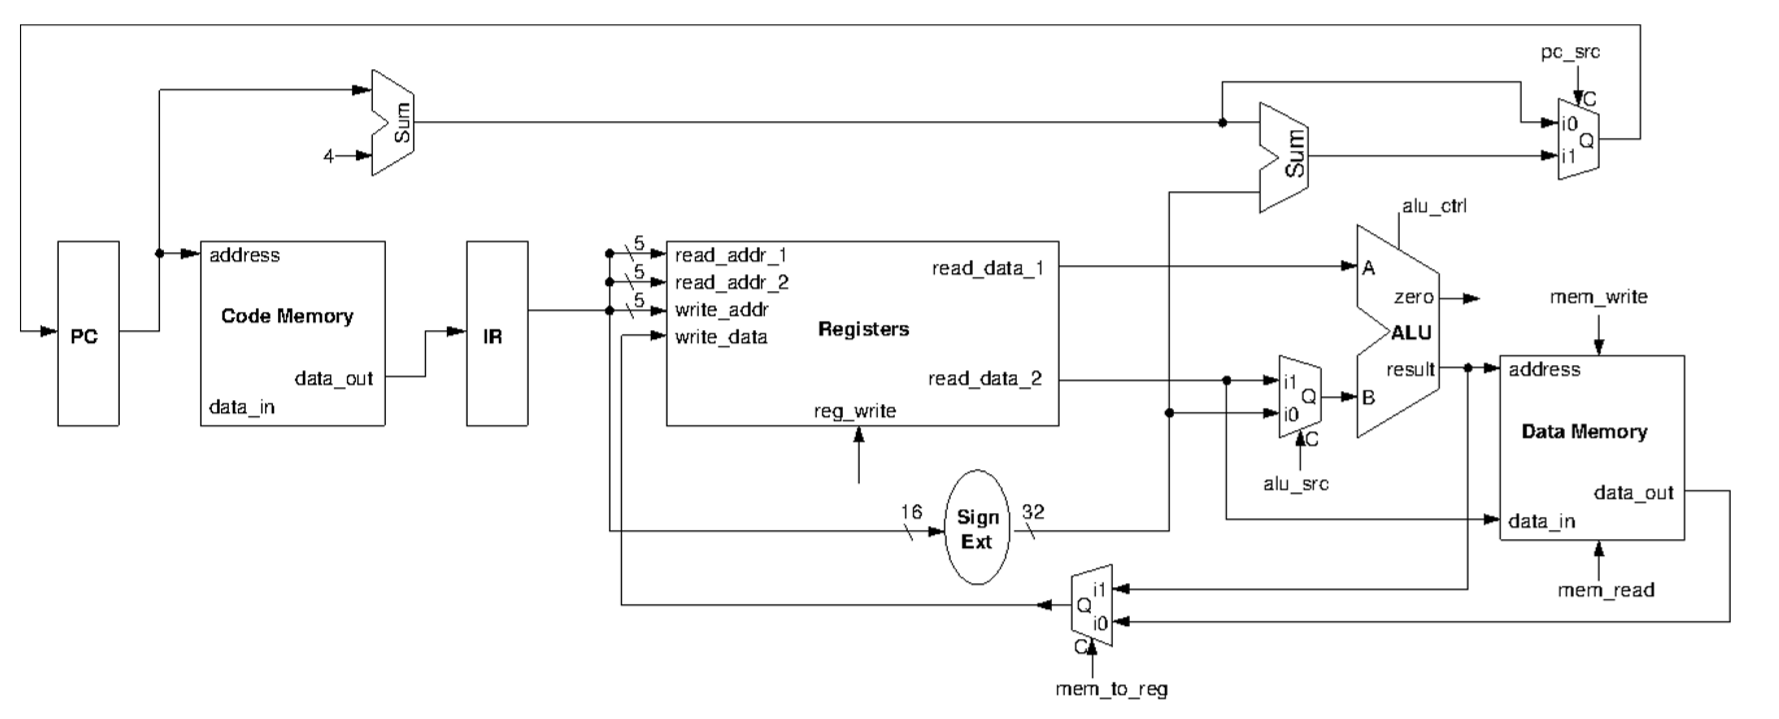
\includegraphics[width=18cm]
		{csa/fullint}}
	\caption{\label{fig:fullint} Mostly integrated MIPS datapath}
\end{figure}

\subsection{Control}
In the datapath there are a few control wires added; the Main Control unit is in charge of decoding the instruction and transmitting the proper control signal. We need to know what each control signal means first.
\begin{itemize}
	\item reg\_write: If true, allows writes to registers
	\item alu\_src: Chooses between register (False) or sign extension unit (True) input for ALU
	\item mem\_to\_reg: Selects whether ALU output (False) or memory (True) is sent to registers
	\item reg\_wsrc: Selects whether registers write\_address is bits [20-16] (True) or [15-11] (False) of the instruction
	\item pc\_src: Selects whether PC+4 (False) or PC+4+branch (True) is sent to PC
	\item jump: If true, sends jump address to PC; if false, sends output to pc\_src to PC
	\item mem\_read: If true, read from memory is permitted
	\item mem\_write: If true, writes to memory are permitted
	\item alu\_op: Control bits for the ALU
\end{itemize}
\begin{figure}[!htb]
	\center{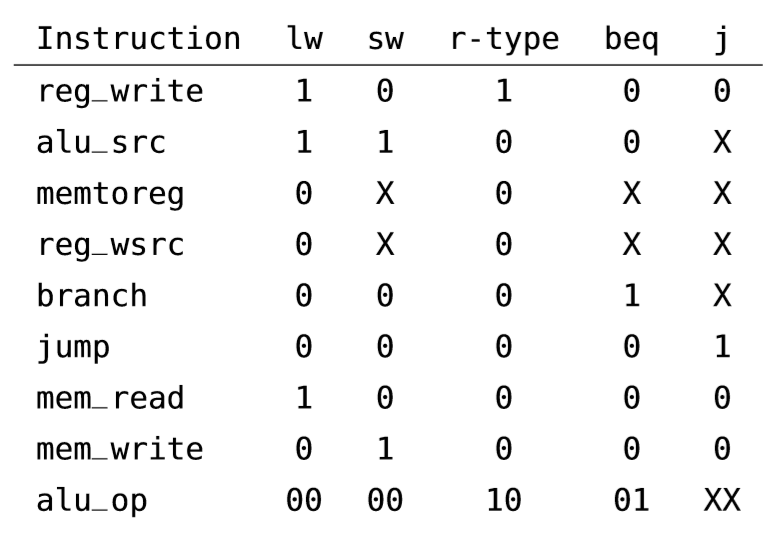
\includegraphics[width=9cm]
		{csa/control}}
	\caption{\label{fig:control} Control Requirements Table per instruction}
\end{figure}
We will look at two ways to implement CPU Control in our every day von Neumanns. We have \textbf{Single Cycle Control} that uses a stateless logic whose input is the 6-bit opcode and whose outputs are the control signals. This is useful if the instructions can be completed in one cycle. In reality though, some operations will take multiple cycles due to the different operations, such as memory access, being slower than others.

\subsection{State Control}
Finite State Machines, rather than being stateless, has, well, states. We learned two ways of implementing them, Mealy states machines and Moore state machines. In a Mealy state machine, the outputs and the next state are a combinatorial function of both the state and the inputs, whilst in a Moore state machine, the outputs are a function of the state only while the next state depends on the inputs and current state. \newline What this means is that the output of a Moore machine can only change on the clock edge, whilst the output of a mealy machine can change asynchronously when the inputs change. Which of these is desirable is based on the application. Here are the main factors to consider when designing a FSM:
\begin{itemize}
	\item Determine how many states are needed and how to enumerate them
	\item Determine the sequence of state transitions
	\item Write down truth tables for the combo logic
	\item Implement the logic
\end{itemize}
\begin{figure}[!htb]
	\center{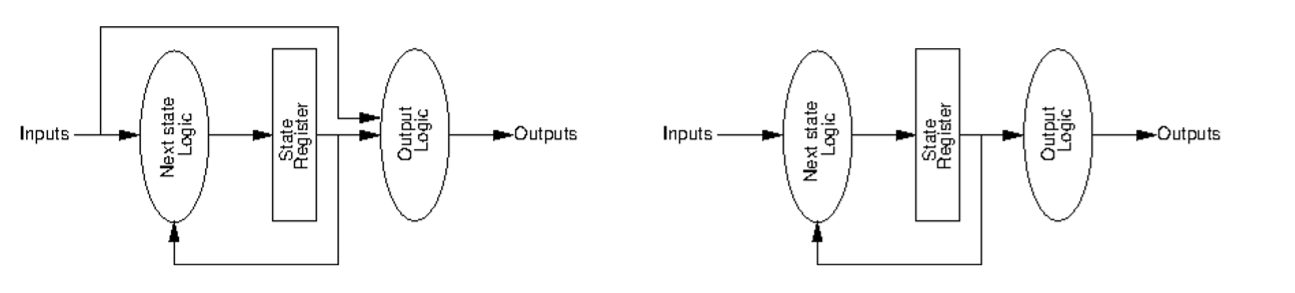
\includegraphics[width=11cm]
		{csa/statemachines}}
	\caption{\label{fig:states} Mealy VS Moore (brawl of the century)}
\end{figure}
In general, these are the major differences between Mealy and Moore.
\begin{enumerate}
	\item Mealy machines tend to have fewer states
	\begin{itemize}
		\item Different outputs on arcs rather then states
	\end{itemize}
	\item Moore machines are safer to use:
	\begin{itemize}
		\item Outputs change at clock edge (delayed one cycle)
		\item In Mealy, only when logic is done is the output changed, causes problems with interconnected machines
	\end{itemize}
	\item Mealy machines react faster to inputs
	\begin{itemize}
		\item React in same cycle, no need to wait for the clock
		\item In moore machines, more logic may be necessary to decode state into outputs; more gates == more delays
	\end{itemize}
\end{enumerate}
\section{Optimisation}
\subsection{Pipelining}
\paragraph{Overview}
Pipelining is defined as (thanks google): a form of computer organization in which successive steps of an instruction sequence are executed in turn by a sequence of modules able to operate concurrently, so that another instruction can be begun before the previous one is finished. Normally, each instruction set is executed before the next one begins. However, we can instead make it where, once a task is finished, the next one is fetched before the original is completed, think in a factory production-line fashion. While each instruction will take the same time (or longer, as all instruction have to be done before any instruction can proceed), the throughput overall is much higher.

\paragraph{MIPS Pipeline}
The MIPS pipeline has registers added to store intermediate results plus any additional control information.
 \begin{figure}[!htb]
	\center{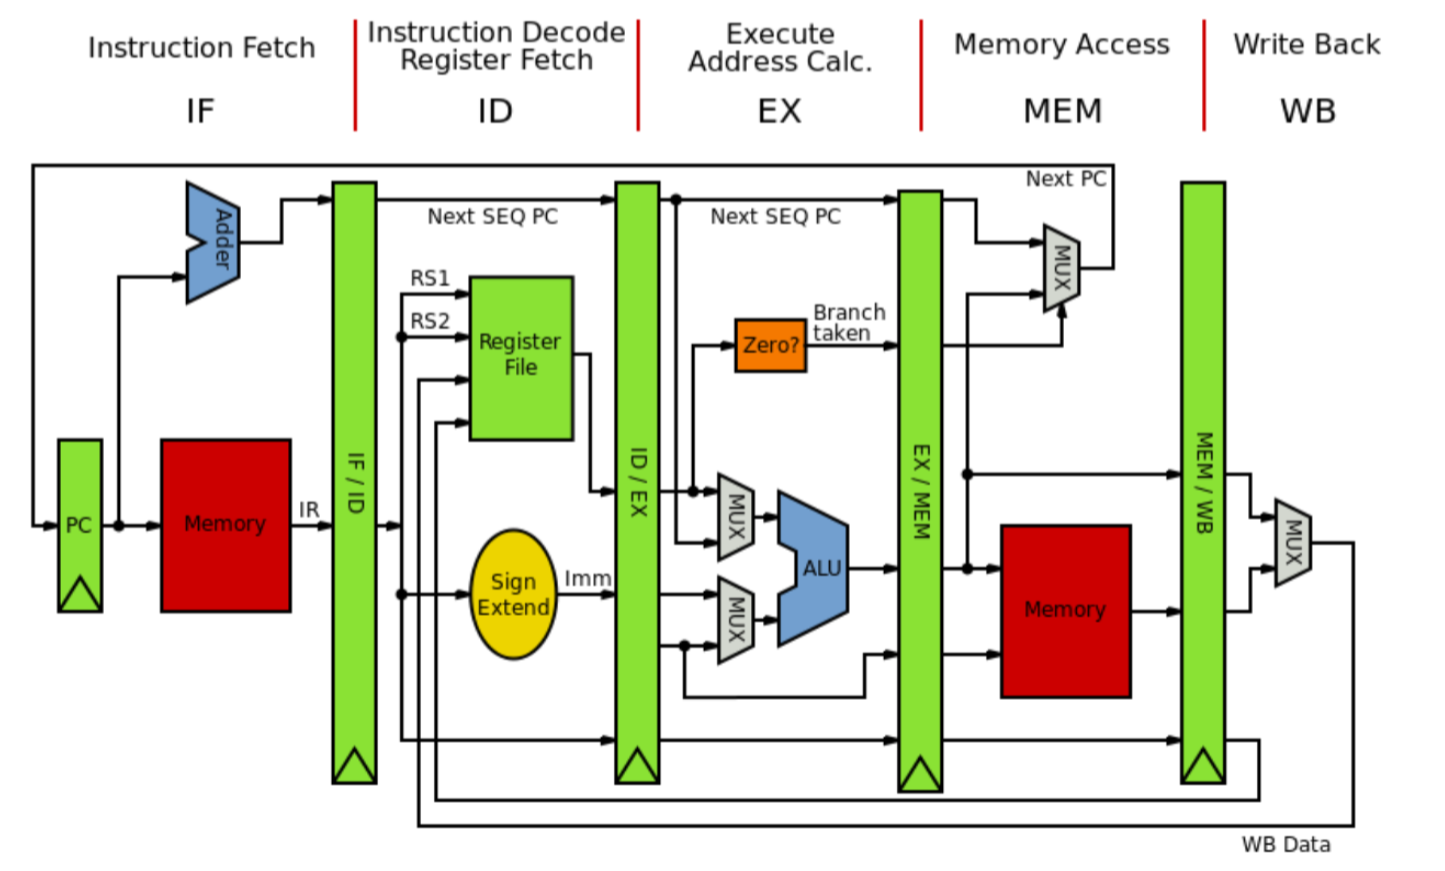
\includegraphics[width=14cm]
		{csa/pipeline}}
	\caption{\label{fig:pipeline} MIPS Datapath Pipeline}
\end{figure}

\subsection{Caches}
\paragraph{Overview}The cache is a moderately fast, medium-sized memory which acts as a buffer between the main memory component and the registers. Caches are used because of the two basic properties of computer programs.
\begin{enumerate}
	\item Spatial Locality: When an item is referenced, you are likely to access nearby items soon.
	\item Temporal locality: When an item is referenced, you are likely to access it again soon.
\end{enumerate}
At the most fundamental level, caches are just a block of memory. However, caches need to store a copy of a value from the main memory and its address in the main memory. This address is often called the cache tag. When the CPU is accessing the main memory, it goes through the cache and compares the tag with the address its looking for. It can either hit or miss; because this check is done every time, a cache will add more time than without a cache on a cache miss.
\paragraph{Cache Associativity} One of the biggest factors affecting cache performance is its degree of associativity. This is the number of different locations that an item of data can occupy in the cache. One of the most common cache designs is the direct-mapped cache AKA one way associative. Data from each address in main memory can only go in one location in the cache, making access time to the cache fast. The way this works is, a subset of the address is hard-coded into the cache (eg. 111xxxx) The remaining bits are checked against the tag for the entry. \newline
The main issue with direct-mapped caches is that two items of the same subset (111x, 111y) cannot be stored simultaneously, resulting in potential thrashing, where entries in a cache continuously swap, destroying any performance benefit you dreamt of. The best way to potentially deal with thrashing is in an n-associative cache, where each address maps to $n$ cache entries (eg. 10, 01) and multiples of them can exist. A cache where the $n$ is the same number of locations in the cache is said to be fully associative. Positive include no thrashing and lower main memory accesses, negatives include slower access time to accommodate for the cache.
\paragraph{Cache Refill Strategies}
Following a cache miss, temporal locality states the new data accessed in the main memory should be moved to the cache. We use a data structure known as least-recently-used (LRU) queue, which removes the lease recently used item when inserting an item to a full list. Ofcourse, this might not be the best plan, but it is up to the designer to figure out the best refill policy as it can different between machines, code, and any other cache usage factor.
\paragraph{Cache Writing Strategies}
Reading from a cache is hit or miss, pretty simple. 
\paragraph{Performance Benefits}
Cache performance is a calculation that is really simple. You take the proportion of instruction time used on on memory access, and convert the amount that would be a hit on the cache to the cache access time, and just like magic, you have the new time. \[T = N(t_{cyc} + m(t_{cache} + (1-h)t_{mem}))\]
\begin{itemize}
	\item $N$ = Number of instructions
	\item $t_{cyc}$ = The cycle time
	\item $t_{mem}$ = Memory cycle time (Additive to cycle time)
	\item $t_{cache}$ = Cache access time
	\item $m$ = The proportion of memory access instructions
	\item $h$ = Cache hitrate
\end{itemize}
\section{Number Representations}
\subsection{Types}
\paragraph{Base Two}
Numbers in computers are represented in binary, base two, format. Normally, our normal understanding of numbers is in Base Ten. \[3 = 1 \times 10^0\] but this can also be represented in Base Two \[3_10 = 11_2 = 1 \times 2^1 + 1 \times 2^0\]. In terms of integers at least, this means that the maximum size we can represent in $n$ bits is \[2^n - 1\] so a 32-bit value is, at most, $2^{32} - 1$.
\paragraph{Representations}
Ofcourse, this method of representation using twos also works for decimals, but where in a byte do we store decimals? In the fixed point representation of real numbers, the decimal is implied. For example, assuming a 16-bit piece of memory, we imply that the integer portion will cover the first 8 bits and the decimal portion the remaining 8 bits. As such, the computer will recognize the values with no manual decimal placed.
Modern computers now use the floating point representation. \[V = M \times 2^E\] Floating point uses a mantissa $M$ and an exponent $E$ to store its values. Part of the bits, for example 4 bits in an 8-bit system, are used to store the mantissa and the rest represent the exponent. In an 8 bit system as a result, you can represent a value like 112 as \[01110111 \rightarrow 0.111 \times 2^{0111}\]
\paragraph{Negative Value}
Negative values are represented using something we like to call Two's Complement. What this simply means is, the left-most bit is "0" for the positive variant. We know that each value we can represent should have a value in the same field that, when added together, form $0$. We represent this negative value by inverting every bit and adding 1 to the LSB. \[ 0101 \rightarrow 1011\]. The system reads the left-most bit as a 1, so we know its negative, the rest follows.

\subsection{Arithmetic}
\begin{figure}[!htb]
	\center{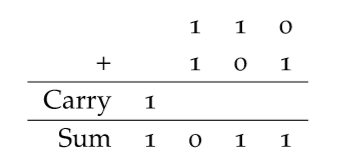
\includegraphics[width=5cm]
		{csa/adding}}
	\caption{\label{fig:adding} Arithmetic example for base 2}
\end{figure}
Adding bits works the same as adding and subtracting the numbers in base 10. For example, if we were to add $0110$ and $0101$, the result would be $1011$ as seen by the figure. When our column adds to a total of 2, a one is carried on column to the right and the 2 becomes a 0. If the total becomes 3, a 1 is still carried, but the column becomes a 1.
For subtraction, you can add the base value and the two's compliment of the other value. This simplifies the process greatly.
\newpage
\subsection{Hex Representation}
\begin{figure}[!htb]
	\center{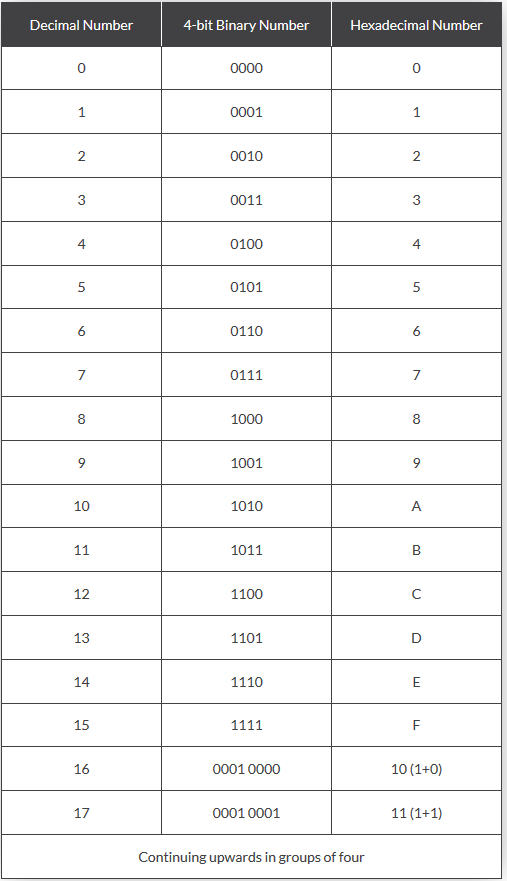
\includegraphics[width=8cm]
		{csa/hex}}
	\caption{\label{fig:adding} Deciaml $\rightarrow$ Binary $\rightarrow$ Hex Representation}
\end{figure}
\section{Logic}
\subsection{Logic Gates}
The basic building block of our CPUs today are transistors. Transistors are made up of three parts, a gate, a source, and a drain. They are used in circuits; it is enough to understand that they are switches that are controlled by the gate voltage.
Transistors process bits (0 voltage and $>$ 0 voltage). The output changes based on how the circuit is built. For example, we have the NOT gate which takes a signal and inverts it on output. For simplicity, gates are drawn in an abbreviated form as seen in Figure \ref{fig:gates}.
\begin{figure}[!htb]
	\center{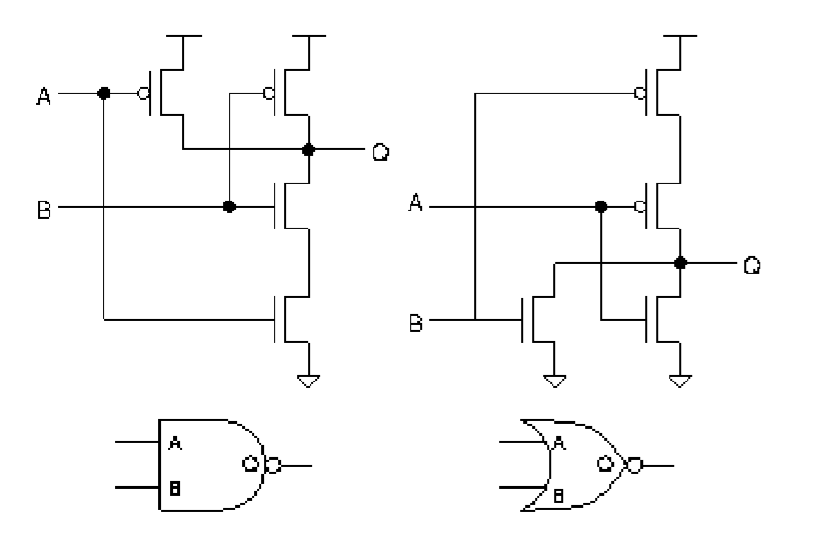
\includegraphics[width=9cm]
		{csa/gates}}
	\caption{\label{fig:gates} NAND and NOR gates}
\end{figure}
If you've done Minecraft Redstone, you might find yourself at home on this section. Sadly real life is a little more complicated.
\paragraph{Combination Logic} A general term for blocks of digital logic which contain no kind of memory. For each $n$ inputs, there are $2^n$ possible output states. Each of these outputs can be represented by a basic boolean algebra (eg. $A\wedge B$) and written into a circuit as such.
\subsection{Latches}
\paragraph{Latch} A latch is a circuit that has two stable states and can be used to store state information. The circuit can be made to change state by signals applied to one or more control inputs, and will have one or two outputs. It is the basic storage element in sequential logic. NAND and NOR (pictured) are "programmable inverters"; cross coupled NAND/NOR gates are used. We will be covering two types, SR (Set-Reset) and D(data/delay).
\begin{figure}[!htb]
	\center{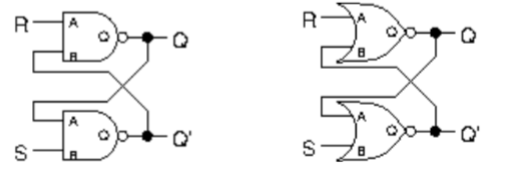
\includegraphics[width=7cm]
		{csa/nandnor}}
	\caption{\label{fig:nandnor} NAND and NOR Crosscoupled}
\end{figure}
\paragraph{RS NOR Latch} The most basic latch is the RS NOR Latch constructed from a pair of cross coupled NOR gates, as pictured. Due to the nature of the setup, R=S=1 should be avoided.
\begin{figure}[!htb]
	\center{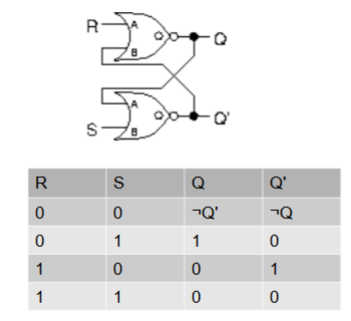
\includegraphics[width=6cm]
		{csa/rsnorlatch}}
	\caption{\label{fig:norlatch} RS NOR Latch}
\end{figure}
\paragraph{D Latch} To avoid the case of R=S=1, we can use a D Latch to change the input into the RS Latch. A simple addition to the circuit removes this issue. At C=0, R=S=0, and C=0, R=$\neg$D and S=D, giving the RS control to the D value.
\begin{figure}[!htb]
	\center{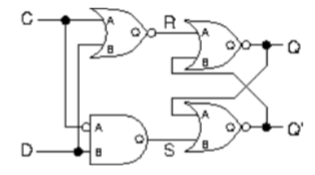
\includegraphics[width=6cm]
		{csa/dlatch}}
	\caption{\label{fig:dlatch} D-Latch}
\end{figure}
\paragraph{Edge Triggered Flip Flop} The RS latch responds to the data inputs (S-R or D) only when the enable input is activated. However, it is desirable to limit the responsiveness of a latch circuit to a very short period of time instead of the entire duration that the enabling input is activated. We can do this using an edge triggered flip flop. By placing some latches with some neat logic, we can obtain this behaviour. The first half becomes transparent at C=0, and the second half at C=1. When C: 0 $\rightarrow$ 1 the second stage "captures" output of the first stage. This way, Q is stable for the whole clock cycle.
\begin{figure}[!htb]
	\center{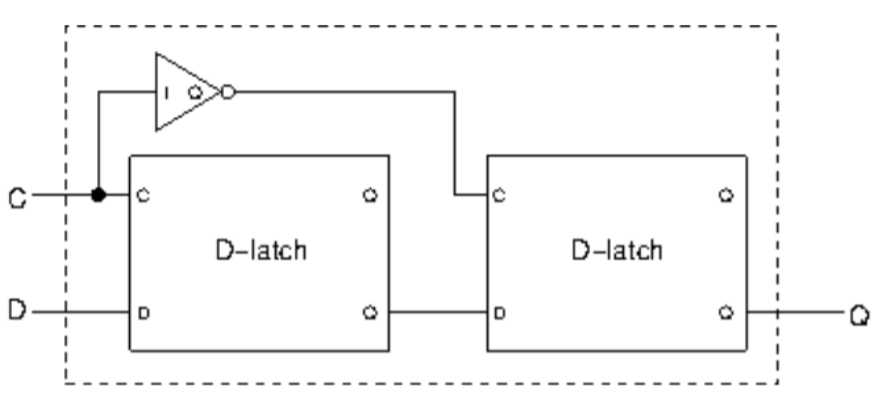
\includegraphics[width=7cm]
		{csa/flipflop}}
	\caption{\label{fig:flipflop} Edge Triggered Flip Flop}
\end{figure}
\subsection{Datapath Components}
\paragraph{Multiplexer Construction} Multiplexers are used commonly in the MIPS datapath. Let's look at the logic of a 2-1 multiplexer with inputs i0, i1 and C with output Q. \[Q = (C \land i1) \lor (\neg C \land i0)\] As you can see, this is a simple construction of two AND gates followed whose outputs are the inputs of an OR gate. For larger bits like 32, we use 32 single-bit multiplexers that share the same selection signal $C$.
\begin{figure}[!htb]
	\center{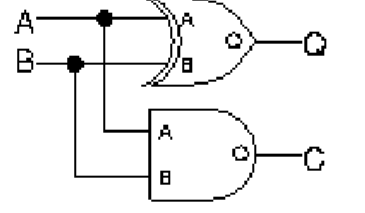
\includegraphics[width=6cm]
		{csa/halfadderlogic}}
	\caption{\label{fig:halfadderlogic} The circuit for a half adders; an XOR outputs the addition and an AND outputs the carry}
\end{figure}
\paragraph{Adders and Half-adders} Thanks to our good friend google, we can find the definition of an adder as a unit which adds together two input variables. A full adder can add a bit carried from another addition as well as the two inputs, whereas a half adder can only add the inputs together, throwing its carry to the shadow realm (a different output signal). When thinking of half adders, we want to find a way to manage handling the carry going in $C_{in}$ and the carry going out $C_{out}$. This can be handled easily by using two half adders and an XOR with the carries from the two adders. We can then use half adders for a 32-bit adder, with two halvess creating one whole. Each bit uses a full adder, and a half adder is used for the LSB, since a carry there indicates an overflow.
\begin{figure}[!htb]
	\center{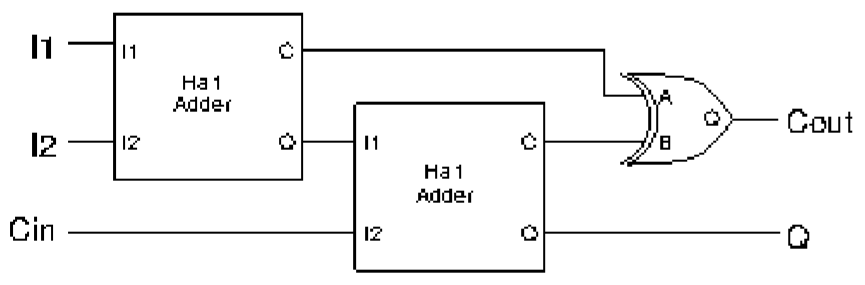
\includegraphics[width=8cm]
		{csa/lsbadder}}
	\caption{\label{fig:lsbadder} The full adder circuit generated from two halves}
\end{figure}
\paragraph{Adder to ALU}
From here, all we do is take our 32-bit adder, stick in some AND and OR gates (to handle the appropriate operation) and some multiplexers to know which operations are required. This creates an ALU.
\begin{figure}[!htb]
	\center{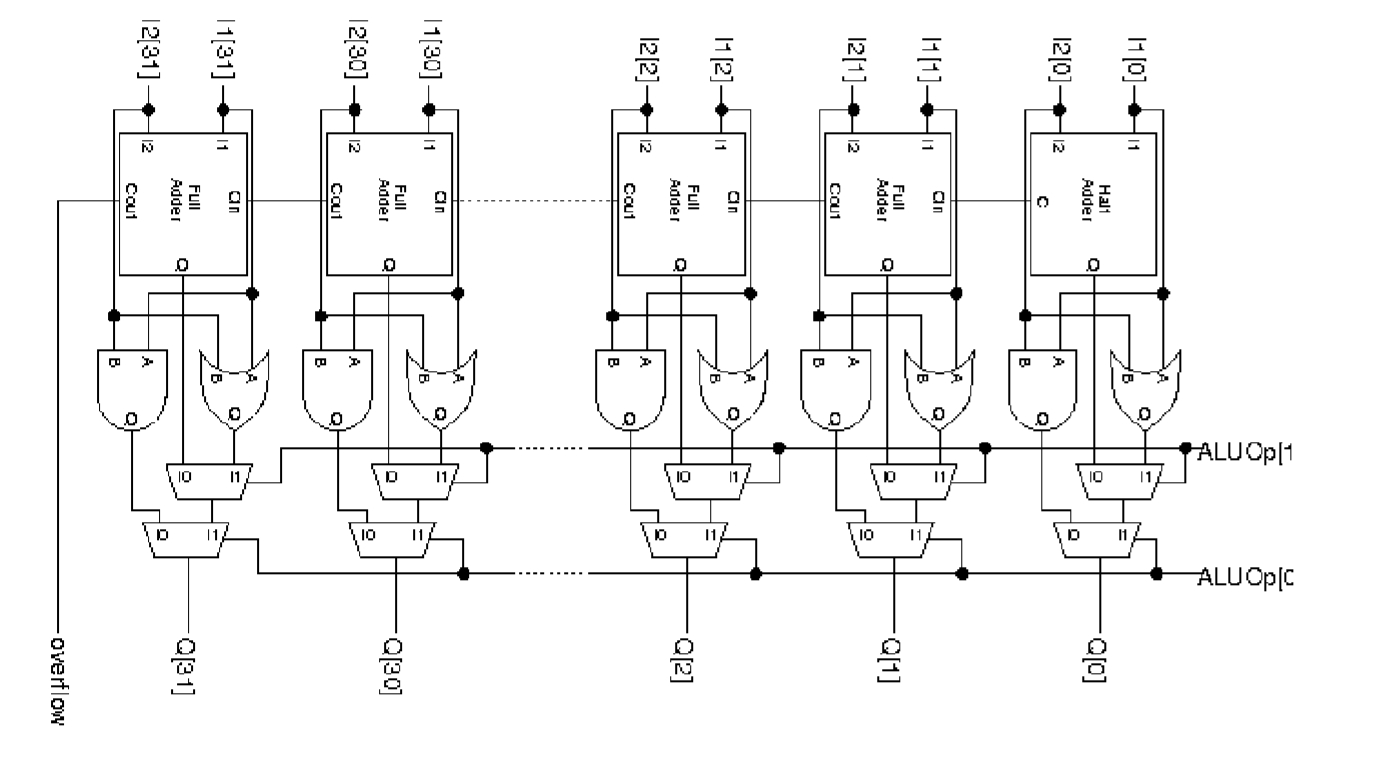
\includegraphics[width=14cm]
		{csa/aluadders}}
	\caption{\label{fig:aluadders} General 32-bit ALU design with the adders}
\end{figure}
